\section{Assemblies of DC1 and Tsth20}

For general assembly metrics of DC1 and Tsth20, the QUAST tool was
used. Results from QUAST are shown in figure~\ref{table:assemblies},
from which we can make several observations. In DC1 and Tsth20, the
total contig counts are an order of magnitude smaller when compared to
the other NCBI RefSeq assemblies, inidicating highly contiguous
assemblies from nextDenovo and nextPolish. This is likely due to the
use of long-read sequencing used in the assemblies of DC1 and
Tsth20. The total assembly lengths are similar, ranging from 38Mb to
42Mb, except in the case of \textit{T. reesei}, which is known to have
a significantly smaller genome length \cite{Kubicek2019} at roughly
33Mb. The largest contig size for each assembly varies greatly. DC1
and Tsth20 have the largest contigs of all assemblies being
considered, which is again likely due to the inclusion of long-read
sequencing data in the assembly process. The N50 values for all
assemblies are above 1Mb, with DC1 and Tsth20 N50s being at minimum
three times larger than others assemblies. Results from this table
indicate that the assemblies of DC1 and Tsth20 are more contiguous
than the assemblies of \textit{Trichoderma reesei, harzianum and
  virens} also considered in this analysis. While contiguity is not
the sole indicator of genome quality, it does provide confidence in
the quality of the input data and resulting assemblies. In general,
the assemblies of DC1 and Tsth20 are of similar length to existing
\textit{Trichoderma} assemblies and the number of contigs reported
match the number of `chromosome' scale contigs reported in other work.

\begin{table}
  \begin{center}
    \begin{tabular}{|c|c|c|c|c|c|c|}
      \hline
      Strain & Total Contigs & Total Length & Largest Contig & GC\% & N50 & L50 \\ \hline
      DC1 & 8 & 38.6 Mb & 11.49 Mb & 47.97 & 5.69 Mb & 3 \\ \hline
      Tsth20 & 7 & 41.58 Mb & 8.02 Mb & 47.33 & 6.52 Mb & 3 \\ \hline
      \textit{T. harzianum} & 532 & 40.98 Mb & 4.08 Mb & 47.61 & 2.41 Mb & 7 \\ \hline
      \textit{T. virens} & 93 & 39.02 Mb & 3.45 Mb & 49.25 & 1.83 Mb & 8 \\ \hline
      \textit{T. reesei} & 77 & 33.39 Mb & 3.75 Mb & 52.82 & 1.21 Mb & 9 \\ \hline
    \end{tabular}
  \end{center}
  \caption{General assembly metrics produced by QUAST (a
    genome quality assement tool).}
  \label{table:assemblies}
\end{table}

During initial investigation of the sequences used as input to the
assembly process, we observed that the reads contained abnormal ratios
of GC content. To see if this observation extended to the assemblies
as well, 250 bp sliding windows were used to calculate GC content for
all assemblies included in this analysis. The results of this analysis
are shown in figure~\ref{fig:assembly-gc}. Of the included assemblies,
anomalous GC content in the form of AT-rich sequences were identified
in DC1, Tsth20, \textit{T. reesei} and \textit{T. harzianum}, with
\textit{T. virens} deviating from the other assemblies showing very
few AT-rich windows. Anomolous GC content is visualized on the left
tails of the distributions with a local peak around sequences
containing 10 percent GC content. In addition to the confirmation of
increased AT-rich sequence content in most assemblies, it appears that
the distribution of GC content in \textit{T. reesei} differs from the
other assemblies. The curve of GC content for \textit{T. reesei},
visualized in green in \ref{fig:assembly-gc}, lies farther to the
right, indicating more GC content, or fewer AT-rich windows, in its
assembly. While the left tail of the curve also shows an increase in
AT rich sequence composition, it is shifted farther right than other
\textit{Trichoderma} assemblies. Investigation of these anomalous
regions is continued in section ...

\begin{figure}
  \begin{center}
    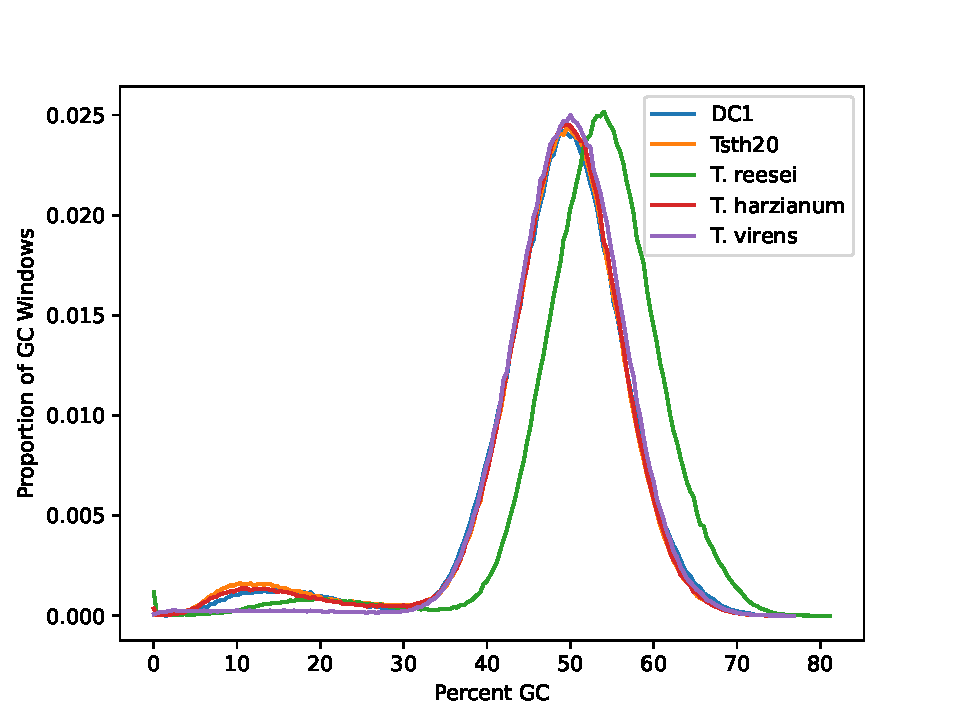
\includegraphics[width=0.8\textwidth]{figures/gc-plot.pdf}
  \end{center}
  \caption{Plots showing the frequency of GC values calculated from
    sliding windows for each assembly.}
  \label{fig:assembly-gc}
\end{figure}


